\title{Simulated Annealing}
\label{chp:simulated-annealing}
\author{Alberto Franzin, Thomas St\"utzle}
\institute{Universit\'e Libre de Bruxelles}
\maketitle

\urldef\supplementurlsa\url{https://github.com/ieee-cis/IEEE-CIS-Open-Access-Book-Volume-1/tree/main/Part%202%20-%20Search-Based%20Optimization/Simulated%20Annealing/SupplementaryMaterial}

\newcommand{\initialtemperature}{\textsc{Initial Temperature}\xspace}
\newcommand{\stoppingcriterion}{\textsc{Stopping Criterion}\xspace}
\newcommand{\explorationcriterion}{\textsc{Neighbourhood Exploration}\xspace}
\newcommand{\acceptancecriterion}{\textsc{Acceptance Criterion}\xspace}
\newcommand{\temperaturelength}{\textsc{Temperature Length}\xspace}
\newcommand{\coolingscheme}{\textsc{Cooling Scheme}\xspace}
\newcommand{\temperaturerestart}{\textsc{Temperature Restart}\xspace}
\newcommand{\initialsolution}{\textsc{Initial Solution}\xspace}
\newcommand{\neighbourhood}{\textsc{Neighbourhood}\xspace}
\newcommand{\brsa}{\texttt{BR1}\xspace}
\newcommand{\qsa}{\texttt{Q8-7}\xspace}

\label{sec:introduction}

The origins of simulated annealing lie in the work of Metropolis 
\textit{et al.} in statistical physics \cite{MetRosRosTel53}, who proposed an algorithm to simulate the displacement of particles in
a solid body. A random displacement is effectively performed (``accepted'')
if it lowers the total energy of the system, while it is performed with 
probability $\exp{(-\Delta E / k_BT)}$ if the energy variation $\Delta E$ is
positive. In the Metropolis formula, $k_B$ is the Boltzmann constant and $T$
is the temperature at which the displacement is evaluated.
For a temperature value $T$, the higher $\Delta E$, the lower the chance
the displacement effectively happens. Likewise, if the given $\Delta E$ is held constant but positive,
the higher the temperature, the higher the probability of the displacement.

In one of the first
instances of algorithmic development inspired by natural phenomena, 
Kirkpatrick, Gelatt and Vecchi \cite{Kirkpatrick83},
and independently \v{C}erny \cite{Cer85}, thought to
view a combinatorial optimization problem as a solid, whose states are the
feasible solutions of the problem. The objective function value of
a particular solution is related to the level of energy of the system in
a particular configuration. The system is first heated
and then cooled little by little until it ``freezes''. 
Out of the metaphor, the algorithm starts from an initial solution
and iteratively evaluates candidate ones.
The temperature used to evaluate an exchange starts at a high value,
and is progressively lowered following a geometric trend. For temperature
values low enough, the probability of accepting worsening moves becomes
effectively zero, and the algorithm behaves like an iterative improvement.


The function originally proposed to determine the acceptance
or the rejection of a move is the so-called \textit{Metropolis criterion} \cite{MetRosRosTel53},
where a solution of equal or better quality is accepted always. If, however, the new solution $\mathbf{x^\prime}$ is worse than 
the current solution $\mathbf{x}$, it is accepted with a probability $\exp{(-(f(\mathbf{x^\prime}) - f(\mathbf{x}))/T)}$ for 
minimization or with a probability $\exp{(f(\mathbf{x^\prime}) - f(\mathbf{x})/T)}$ for maximization problems, where $f(\cdot)$ is the objective function. 
Here, we always will assume minimization problems; it is straightforward 
to adapt the algorithm for a maximization problem.
The probability of accepting worsening moves depends 
on the relative worsening in terms of
solution quality from the incumbent one and on the scalar parameter $T$, called \textit{temperature}.
For a proposed worsening move, high values of the temperature parameter provide a higher chance of 
accepting it than lower values. High temperature values therefore promote a stronger exploration behaviour,
while low values are associated to a strong exploitation.
Simulated annealing can thus be considered as a local search with 
a diversification mechanism governed by the temperature parameter.

The choice of the value for the temperature parameter is crucial in obtaining good results. 
The original formulation, the conventions and the folklore deriving
from the annealing metaphor, but
also the theoretical works on simulated annealing, make use of a sequence of values.
In general, the temperature value is set at a ``high'' initial value,
and progressively decreased to a final ``low'' value, to make
the algorithm transition from a highly exploration behaviour to a converging,
exploitative one. Optionally, the temperature value is raised again or restored
to its initial value, to promote a cycle of diversification and intensification
phases.

Immediately after its introduction, simulated annealing attracted the attention of 
several researchers, thanks to its simple formulation and the quality
of the results obtained in several works. 
It became therefore one of the most popular algorithms for combinatorial
optimization problems, and it has been used in thousands of works.
Along with its use, researchers became interested in modeling its behaviour from
a theoretical perspective. A series of works, mostly in the 80s' and early 90s',
focused on conditions for the cooling scheme to obtain the optimal solution for a
given problem and instance, mostly under unrealistic conditions such as an
infinite number of evaluations \cite{GemGem1984,LundyMees1986,Hajek1988,RomSan1991}. 
Yet, by simply enumerating the
search space one could guarantee to find the optimal solution even in
finite time but, in the end, very large time which is usually infeasible.  
Thus, a more important question would refer to the
convergence speed of simulated annealing, that is, how quickly good solutions are found; yet, results addressing this
question are rare. Also, practical annealing schedules decrease the
temperature much faster than what is implied by the theoretical results and
therefore the convergence proofs do not apply in this case. 

In this chapter we summarize research on simulated annealing and its behaviour.
We show how implementing a simulated annealing algorithm can be seen as a configuration task,
and makes use of efficient artificial intelligence tools to automatically generate high-performing
algorithms for different scenarios. We then explore quickly the results and the algorithms we 
obtain and then conclude the chapter.



\section{A simulated annealing algorithm}

\subsection{A basic simulated annealing algorithm}


Implementing a basic simulated annealing algorithm is quite fast. First, one needs a starting 
solution, which can be a uniformly random solution in the simplest case, or one computed using a simple heuristic
like a constructive one. 
Second, one needs a neighbourhood, which is an essential ingredient. 
Sometimes the neighbourhood can be more complicated as 
for some problems one needs to have various neighbourhoods and decide how to schedule them. Then one has to choose a 
simulated annealing acceptance criterion. As the simplest one,
use the Metropolis criterion, which we have detailed in the introduction of this chapter
 \cite{MetRosRosTel53,JohAraMcGSch1989,JohAraMcGSch1991}. As a reminder, an 
improving or equal move is always accepted and a worsening one is accepted with a probability 
$\exp{(-(f(\mathbf{x^\prime}) - f(\mathbf{x}))/T)}$. The rest is embedding the annealing criterion in an 
\textit{annealing schedule}, which is also called \textit{cooling schedule}. 
It is defined by an initial temperature $T_0$, a scheme saying how the new temperature is
obtained from the previous one, the number of search steps to be performed at
each temperature, and a termination condition. A common choice is in simulated annealing to use
a geometric cooling, which is that  $T_{i+1} = \alpha T_i$, where $\alpha$ is a parameter 
with $0 < \alpha < 1$. This operation, called annealing step, is usually done 
after a number of search steps (that is, candidate solution evaluations) performed at 
the same temperature, often for a number of evaluations that is a multiple of the neighbourhood size. 
Finally the termination criterion is often based on the acceptance ratio, that is, 
the ratio of proposed steps versus the accepted steps. 

\subsection{A component-based overview of simulated annealing}
\label{sec:sacomponents}

To use a full-fledged simulated annealing one has to set still 
the control parameters, such as the initial temperature value,
the temperature update factor, or the number of moves to be evaluated at the same temperature.
We have now a somewhat reasonable algorithm and
in the meantime, with the thousands of papers, much more involved 
simulated annealing algorithms have been proposed. So in 
\cite{FraStu2019:cor}, we identified a total 
of seven components, whose function and connection
define what a simulated annealing is, and how it works. Two other components 
are necessary to elaborate information for the specific problem considered,
and are not unique to simulated annealing. Problem-specific components can be considered as 
inputs to simulated annealing.
The outline is given in Algorithm \ref{algo:simannealing}, and the components
are subsequently described.

\begin{algorithm}[ht!]
	  \caption{Component-based formulation of SA. The components we
      have identified for our analysis are written in \textsc{Smallcaps}.}
     \label{algo:simannealing}
    
    Parameters: a problem instance $\mathcal{I}$, a \neighbourhood $\mathcal{N}$ for the solutions, an \initialsolution $\mathbf{x}_0$, control parameters
    
    Output: the best solution $\mathbf{x^*}$ found during the search.
    
	\begin{algorithmic}[1] 
		\STATE{$\textrm{best solution } \mathbf{x^*} := \textrm{incumbent solution } \mathbf{\hat{x}} := \mathbf{x}_0$\;}
		\STATE{$i := 0$\;}
        \STATE{Initialize temperature $T_0$ according to \initialtemperature\;}
		\WHILE{\stoppingcriterion is not met}
		\STATE{choose a solution $\mathbf{x}_{i+1}$ in the \neighbourhood of $\mathbf{\hat{x}}$ according to \explorationcriterion criterion\;}
		\IF{$\mathbf{x}_{i+1}$ meets \acceptancecriterion}
		\STATE{$\mathbf{\hat{x}} := \mathbf{x}_{i+1}$\;}
		\IF{$\mathbf{\hat{x}}$ improves over $\mathbf{x^*}$}
		\STATE{$\mathbf{x^*} := \mathbf{\hat{x}}$\;}
		\ENDIF
		\ENDIF
		\IF{\temperaturelength is met}
		\STATE{update temperature according to \coolingscheme\;}
		\STATE{reset temperature according to \temperaturerestart scheme\;}
		\ENDIF
		\STATE{$i := i + 1$\;}
		\ENDWHILE
        \STATE{return $\mathbf{x^*}$\;}
	\end{algorithmic}
	
\end{algorithm}

{\initialtemperature.}
The initial value of the temperature parameter, and, usually, the
maximum value the temperature will take. It also defines the maximum amount of 
diversification, that is, how likely the algorithm is to accept worsening moves,
and it is therefore best computed starting from instance characteristics. 
For example, the initial temperature can be set proportionally to the initial solution value, 
or computed according to some search space statistics such as the maximum gap 
or the average gap between consecutive moves computed during a preliminary random walk.

{\initialsolution (problem-specific).}
Simulated annealing starts from an initial solution that has to be provided 
by a problem-specific component, for example, using a
constructive heuristic, another local search, or even a
random solution. Anyway, if one starts from a problem-specific, 
good candidate solution one should use a low temperature start, since 
otherwise the initial solutions gets destroyed. 

{\neighbourhood (problem-specific).}
The neighbourhood function generates the solutions that are at
distance of one move from the incumbent one. This is also the
component that deals with constraints when necessary, repairing 
infeasible solutions or ensuring that the candidate solutions
generated are feasible. In the simplified environment this is one 
neighbourhood, but it may be that for other problems various 
neighbourhoods are important. 

{\explorationcriterion.}
This component is devoted to selecting one candidate solution to evaluate for acceptance, in the neighbourhood
of the incumbent one. The traditional simulated annealing uses the random selection of a neighbour solution, but alternative
schemes are possible, such as a sequential evaluation following an enumeration
of the solution in the neighbourhood, or even mini-local searches \cite{COnnolly1990,IshMisTan1995}.

%\paragraph
{\acceptancecriterion.} 
The function that determines whether the solution selected by the 
\explorationcriterion should be accepted and replace the incumbent.
The traditional and most popular criterion is the Metropolis condition described at the beginning of this chapter,
but several other criteria have been proposed.
Notably, the Threshold Acceptance is a deterministic variant of simulated annealing 
that always accepts candidate moves that worsen the solution quality of an amount bounded by the temperature value
\cite{DueSch90,MosFon1990}. The Late Acceptance Hill Climbing can also 
be considered as an acceptance criterion that can be fit in the simulated annealing 
structure \cite{BurByk2017}. This latter scheme maintains a history of accepted moves,
and always accepts a candidate solution that is improving over either
the incumbent one, or the incumbent solution of $\kappa$ iterations before.

%\paragraph
{\coolingscheme.}
The function that controls the decrease of the temperature parameter.
The original simulated annealing papers use a geometric criterion, that decreases the temperature
value by a multiplicative factor $\alpha \in (0,1)$, i.e. $T_{i+1}=\alpha T_i$, with $\alpha$ constant throughout
the whole search \cite{Kirkpatrick83,Cer85}. In accordance with the annealing metaphor and the idea of
transitioning from exploration to exploitation, cooling schemes generally yield
monotonically decreasing sequences of temperature values. Some authors have,
however, deviated from the annealing behaviour and proposed schemes that
always keep the same temperature value, or have the temperature value
``fluctuate'', allowing for phases of both controlled increase and decrease
of the temperature parameter \cite{HuKahTsa95}. 
This fluctuation is intended to exhibit a behaviour similar to a fixed temperature value,
while at the same time promoting alternating phases of limited exploration and exploitation,
thus bridging the two opposite SA behaviours.

%\paragraph
{\temperaturelength.}
This component controls the amount of candidate solutions that will be
evaluated using the same temperature value; in other words, it determines when
the \coolingscheme should be used.
The simplest options are constant values, either absolute or proportional to 
some problem characteristic such as instance or neighbourhood size
\cite{HusStu2014cor,JajMinHarPro1992}. However, 
adaptive schemes that make the decision on when to update the temperature 
based on the outcome of the search (for example, a certain amount of accepted moves \cite{Abramson1991})
can provide a more fine-grained control of the exploration/exploitation
trade-off.

%\paragraph
{\temperaturerestart.}
This component determines if and when the temperature value
should be reset to its original value, or set to another higher value (reheat).
Its purpose is to promote a new phase of exploration once the temperature has 
decreased enough to void its diversification potential.
As for the \temperaturelength there are many possibilities, both constant and
adaptive \cite{Kirkpatrick1984,AbrAmoDan1999}.

{\stoppingcriterion.}
The last algorithmic component determines when the search terminates.
This can be set according to fixed conditions such as a given runtime
or amount of moves evaluated, or adaptive conditions such as a too low
acceptance rate \cite{JohAraMcGSch1989,JohAraMcGSch1991}.


\subsection{Composing efficient simulated annealing algorithms}
To implement a new or existing simulated annealing, the developer needs
to face several choices. First of all, 
it is necessary to define the choices
that are related to the specific problem considered, that is, an initial
solution from where to start the search, and the neighbourhood function
used to generate new candidate solutions.
Then the search components, that determine how to select a new candidate
solution, whether to accept it, and how to update the control parameters
have to be implemented.

Since the structure of SA is fixed, designing a simulated annealing algorithm
means to choose which components and which numerical parameters
to use. 
A good starting point to determine which choices to make is the existing body of literature.
Even when limiting ourselves to the algorithm-specific components,
we can find plenty of options for each one of them. 

\begin{table}[tb]
    \centering
    \caption{List of options we implemented for the algorithmic components of simulated annealing. 
    Several of these components include additional numerical parameters. 
    For a more formal description of each component and their implementation we refer to \cite{FraStu2019:cor}.}
    \begin{tabular}{l p{8.2cm}}
       \initialtemperature  & Fixed value; proportional to initial solution value; proportional to maximum gap in random walk; proportional to average gap in random walk; Connolly initial temperature scheme;  Misevicius initial temperature scheme; simplified Misevicius initial temperature scheme. \\
    \explorationcriterion  & Random; sequential; Ishibuchi-Misaki-Tanaka 1; Ishibuchi-Misaki-Tanaka 2. \\
    \acceptancecriterion & Metropolis; bounded Metropolis; precomputed Metropolis; Generalized simulated annealing; geometric acceptance; Threshold acceptance; Great Deluge; Record-to-Record; Late Acceptance Hill Climbing; Hill Climbing.\\
    \coolingscheme & Geometric 1; geometric 2; Lundy-Mees 1; Lundy-Mees 2;
    Q8-7; quadratic; arithmetic; no cooling; temperature band. \\
    \temperaturelength & Fixed; \# moves proportional to problem size; proportional to neighbourhood size; \# of accepted moves; bounded (\# accepted moves, max \# moves); arithmetic increase; geometric increase; logarithmic increase; exponential increase.\\
    \temperaturerestart & Never; Restart or reheat based on: \# moves; minimum temperature value; \% of initial temperature value; global acceptance rate; acceptance rate in the last moves; no recently accepted moves. \\
    \stoppingcriterion & runtime; \# moves; minimum temperature; \# cooling steps; \# temperature restarts; \# moves with no accepted solution; global acceptance rate; most recent acceptance rate; no new recent best solution.\\
    \end{tabular}
    \label{tab:options}
\end{table}

In \cite{FraPerStu2018ol} we collected a total of 66 different options for all the
components, reported in Table \ref{tab:options}, which are enough 
to assemble millions of valid simulated annealing
algorithms. Many of those components have their own set
of numerical parameters to choose \cite{HutHooLey2011lion,LopDubPerStuBir2016irace}. 

The traditional, manual implementation of an algorithm is effectively
an exploration of the space of possible valid algorithms. Finding the one
that performs the best over the entire application space (i.e. the whole test set)
is clearly a daunting task.
Developers therefore often revert on results from the
literature and on established practices and conventions. The first 
reasonable algorithm, either assembled or found in the literature,
is then fine-tuned on a limited set of instances.

Aside from being tedious, this process has several drawbacks. 
First, the combination of components and parameters raises a
complex interaction that is often unexpected
to the user. The developer is then forced to evaluate a restricted set of
options on a limited set of instances, thus prioritizing the
algorithmic solutions already explored in past applications and
in the literature. The bias that follows from this process
likely results in sub-optimal algorithms, whose behaviour and
results are unexplained.

In this chapter we demonstrate how the use of powerful algorithm
engineering tools is beneficial in automatically designing simulated annealing
algorithms that can outperform manually designed ones.
We follow the Programming by Optimization philosophy
that envisages increasing levels of automation of the development process
\cite{Hoos:PbO}. 
The implementation of an algorithms moves away
from a purely manual task, to one that relies on automatic tools
to improve existing algorithms, towards an automatic design of new algorithms.

This task can be framed as a machine learning one
\cite{Birattari09tuning}. In a nutshell, our goal is to find 
the parameter configuration that obtains the best results on a \textit{test set} 
of instances, that ideally represent a realistic practical application. 
In absence of an explicitely structured knowledge on the relationship
between configurations and instance characteristics in terms of results, 
we employ a \textit{training set} of instances, different from the test set 
but belonging to the same distribution. On this training set we 
select the configuration with the best results overall.
For more detailed instructions we refer to the existing literature, 
e.g. \cite{Hoos:PbO,MasLopDubStu2014cor,StuLop2019hb,PagStu2019:ejor} in general,
and \cite{FraStu2019:cor} for SA specifically.



\section{Experiments}
\label{sec:exp}


\subsection{Materials and methods}\label{sec:material}
We consider the Quadratic Assignment Problem (QAP), one of the classic NP-hard
problems where we want to find the assignment of $n$ facilities to $n$ locations
with the minimal cost \cite{KooBec57}. A QAP instance is defined by two
matrices, one with the distances $D_{k,l}$ between two locations $k$ and $l$, and
one with the flows $F_{i,j}$ between two facilities $i$ and $j$.
We represent a solution as a permutation $\pi$, whose
elements $\pi(i)$ contain the location of facility $i$. The objective function is
\begin{equation}
  \min\sum_{i=1}^n\sum_{j=1}^n F_{ij} D_{{\pi(i)}{\pi(j)}}.
\end{equation}

We use two groups of different QAP instances. In the first one the distance matrices 
define a structure in the landscape, and we refer to it as the class of \textit{structured} instances. 
In the second one, instead, the matrices are generated
uniformly at random, and we call this the \textit{random} instances class.
Each class
contains $100$ instances of sizes $60$, $80$ and $100$, equally partitioned into
a training set and a test set.
The training set is used to automatically configure 
and design the algorithms using irace, and the test set is used to 
evaluate the configurations obtained, whose results are reported
in the rest of this section.
Every simulated annealing execution runs for ten seconds.
We use the EMILI framework,
where we implemented 66 components and the relative numerical parameters,
for a total of 100 configurable parameters \cite{PagStu2019:ejor}.
We use a budget of $2000$ experiments to configure the numerical parameters
of two existing simulated annealing algorithms, and we automatically design simulated annealing algorithms
using $10$K, $20$K, $40$K and $80$K experiments, where one experiment is a SA run.
The experiments are done on a machine with two Intel Xeon E5-2680v3 CPUs 
at 2.5GHz with 16MB cache, with 2.4GB of RAM available for each experiment.

The algorithm configurator irace implements the iterated racing algorithm 
in an easy-to-use \texttt{R} package
\cite{LopDubPerStuBir2016irace,BirStuPaqVar02:gecco,MarMoo1997air}. 
The basic idea is to spend computational budget only on configurations
that are worth evaluating, rather than waste it on poor ones.
To configure an algorithm it requires only the definition of the parameters,
a training set of instances, and a script that executes the algorithm with 
a list of command-line parameters (provided by irace as input to the script) 
and returns a measure of the quality of the configuration observed on the instance. 
Such metric defines the configuration task as an optimization problem, and commonly 
used ones include the solution quality found by heuristic algorithms, 
or the runtime needed to find the optimal solution.
irace starts from a set of random configurations, and begins to evaluate all of them 
on the training instances, sequentially. The configurations are ranked for each instance, 
based on the results reported. After a few instances, irace begins to discard the configurations 
that perform statistically worse than the best ones, and proceeds to evaluate only the surviving ones. 
This process of configuration evaluation and statistical test, called \textit{race}, 
is iterated until either the budget for evaluations is exhausted, or a minimum number 
of surviving configuration remains. At this point, new configurations are sampled, 
with parameter values around the surviving configurations, and a new race takes place. 
Race after race, the new configurations get sampled increasingly closer to the last best ones.
When the total evaluation budget is terminated, irace returns to the user the best configurations found.

EMILI is a \texttt{C++} algorithmic framework for the development of modular 
stochastic local search algorithms \cite{PagStu2019:ejor}.
Algorithms are instantiated at runtime by selecting the desired combination of 
command-line parameters, that determine which components and numerical parameters 
are selected, and how they are combined.
The modular structure of EMILI makes it possible to design algorithms
bottom-up, so, in principle, of any shape.
However, its flexibility can of course be exploited to design algorithms 
of a given structure, as we do in this chapter by requiring the components 
to be placed in their proper place in the template of simulated annealing
in Algorithm \ref{algo:simannealing}.

\subsection{Simulated annealing algorithms for the QAP}
\label{sec:expsqap}

We start by reproducing two of the many simulated annealing algorithms
proposed for QAP. These algorithms are called \brsa and \qsa
\cite{BurRen1984,COnnolly1990}. 
The only common algorithmic component between the two algorithms is the Metropolis
acceptance criterion. 
\brsa  starts from an initial temperature computed as the maximum gap observed between
consecutive solutions in a random walk \cite{BurRen1984}.
It uses the random exploration of the neighbourhood to select a move to evaluate.
The temperature is updated with a geometric cooling scheme with coefficient $0.5$
every $2 \times n$ proposed moves, where $n$ is the problem size, and restarted 
to its original value after $|N(\mathbf{x})|$ moves, that is, the size of the neighbourhood.
\brsa therefore performs only a few but substantial temperature updates.
In its original formulation, \brsa terminates its search after $10$ temperature
restarts.

The \qsa algorithm from \cite{COnnolly1990} 
uses a custom mechanism to define the initial temperature, relating it to
the final one.
This algorithm uses a sequential exploration of the neighbourhood to select candidate moves,
imposing an order on the solutions in the neighbourhood and following it.
One particular characteristic of this algorithm is the \texttt{Q8-7} cooling scheme,
an adaptation of the Lundy-Mees cooling scheme \cite{LundyMees1986}. After the cooling phase, once $m$
consecutive moves have been rejected, this scheme restores the temperature to the value at which
the current best solution was found, forces the acceptance of the current 
proposed move, and stops the temperature update, keeping the same value until the end of the search.
The $m$ parameter is set proportionally
to the total number of moves evaluated by the algorithm.
During the initial cooling phase of the \texttt{Q8-7}, the temperature is lowered 
after every move evaluated, and there is no temperature restart.
The algorithm as reimplemented from the original paper terminates after
$50 \times |N(\mathbf{x})|$ moves.

Both algorithms start from a randomly generated permutation, and use the
$2$-exchange neighbourhood
\begin{equation}
  \mathcal{N}(\pi) = \{\pi'\:|\: \pi'(j) = \pi(h) \wedge
  \pi'(h) = \pi(j) \wedge \forall l \notin \{j,h\}\: :\pi'(l)
  = \pi(l) \} 
\end{equation}
that swaps two elements in positions $i$ and $j$ in a solution $\pi$. In total, \brsa has five tunable numerical parameters, 
while \qsa has six; as we will not tune the termination condition, this number reduces 
to respectively four and five. The pseudocode for \brsa and \qsa is reported, respectively, in Algorithms 
\ref{algo:brsa} and \ref{algo:qsa}.

\begin{algorithm}[ht!]

	  \caption{Component-based formulation of \brsa with its original parameters. 
	  The components are highlighted in \textit{italic}. The 
      tuned numerical parameters we obtained are: 
      $\theta^\prime = (k = 8.979, \beta = 51, \alpha = 0.9163, \gamma = 83)$ 
      for the structured instances and $\theta^\prime = (k = 6.3173, 
      \beta = 94, \alpha = 0.9206, \gamma = 79)$ for the random instances, 
      and the termination is replaced with a time-based one ($10$ seconds).}
     \label{algo:brsa}
    
    Parameters: a problem instance $\mathcal{I}$, the \textit{$2$-exchange neighbourhood}, 
    \textit{a random permutation $\mathbf{x}_0$}, control parameters 
    $\theta = (k = 1, t = 10, \beta = 2, \alpha = 0.5, \gamma = 1)$
    
    Output: the best solution $\mathbf{x^*}$ found during the search.
    
	\begin{algorithmic}[1] 
		\STATE{$\textrm{best solution } \mathbf{x^*} := \textrm{incumbent solution } \mathbf{\hat{x}} := \mathbf{x}_0$\;}
		\STATE{$i := 0$\;}
        \STATE{Initialize temperature $T_0$ as \textit{the max gap between consecutive solutions in a random walk of length $l=10^4$, with a scaling factor $k$} \;}
		\WHILE{\textit{less than $t$ temperature restarts have happened}}
		\STATE{choose a solution $\mathbf{x}_{i+1}$ in the \textit{$2$-exchange neighbourhood} of $ \mathbf{\hat{x}}$ \textit{at random}\;}
		\IF{$ \mathbf{x}_{i+1}$ meets \textit{Metropolis criterion}}
		\STATE{$ \mathbf{\hat{x}} := \mathbf{x}_{i+1}$\;}
		\IF{$ \mathbf{\hat{x}}$ improves over $\mathbf{x^*}$}
		\STATE{$\mathbf{x^*} :=  \mathbf{\hat{x}}$\;}
		\ENDIF
		\ENDIF
		\IF{$\beta$ \textit{times the instance size number of moves have been evaluated}}
		\STATE{update temperature according to \textit{geometric cooling with factor} $\alpha$\;}
		\STATE{reset temperature \textit{to initial value $\gamma$ times the neighbourhood size}\;}
		\ENDIF
		\STATE{$i := i + 1$\;}
		\ENDWHILE
        \STATE{return $\mathbf{x^*}$\;}
	\end{algorithmic}
	
\end{algorithm}
\begin{algorithm}[ht!]
	  \caption{Component-based formulation of \qsa with its original parameters. 
	  The components are highlighted in \textit{italic}. The 
      tuned numerical parameters we obtained are: $\theta^\prime = (k = 6.7411, 
      \alpha = 0.9114, \beta = 0.2183, m = 600676, j = 97)$ for the structured instances and 
      $\theta^\prime = (k = 5.5683, \alpha = 0.8597, \beta = 0.04, m = 234615, j = 76)$ 
      for the random instances, and the termination is replaced with a time-based one ($10$ seconds).}
     \label{algo:qsa}
    
    Parameters: a problem instance $\mathcal{I}$, the \textit{$2$-exchange neighbourhood}, 
    \textit{a random permutation $\mathbf{x}_0$}, control parameters 
    $\theta = (k = 1, t = 10, \alpha = 1, \beta = 1, m = |N(s)|, j = 1)$
    
    Output: the best solution $\mathbf{x^*}$ found during the search.
    
	\begin{algorithmic}[1] 
		\STATE{$\textrm{best solution } \mathbf{x^*} := \textrm{incumbent solution } \mathbf{\hat{x}} := \mathbf{x}_0$\;}
		\STATE{$i := 0$\;}
        \STATE{Initialize temperature $T_0$ according to \textit{custom formula \cite{COnnolly1990}, with scaling factor $k$} \;}
		\WHILE{\textit{less than $t\times |N(\mathbf{x})|$ moves} have been evaluated}
		\STATE{choose a solution $\mathbf{x}_{i+1}$ in the \textit{$2$-exchange neighbourhood} of $\mathbf{\hat{x}}$ using a \textit{sequential neighbourhood exploration}\;}
		\IF{$ \mathbf{x}_{i+1}$ meets \textit{Metropolis criterion}}
		\STATE{$ \mathbf{\hat{x}} := \mathbf{x}_{i+1}$\;}
		\IF{$ \mathbf{\hat{x}}$ improves over $\mathbf{x^*}$}
		\STATE{$\mathbf{x^*} :=  \mathbf{\hat{x}}$\;}
		\ENDIF
		\ENDIF
		\IF{\textit{$j$ moves have been evaluated}}
		\STATE{update temperature according to \textit{Q8-7 cooling scheme with parameters $\alpha$, $\beta$, $m$}\;}
		\STATE{\textit{never} reset temperature\;}
		\ENDIF
		\STATE{$i := i + 1$\;}
		\ENDWHILE
        \STATE{return $\mathbf{x^*}$\;}
	\end{algorithmic}
	
\end{algorithm}

\subsubsection{Reinstantiating and improving existing algorithms} 
We start with three types of experiments.
In the first one we run the algorithms using their original parameter settings, including the
termination (thus resulting in different running times);
in the second one we take the original parameters but force each algorithm to run for 10 seconds; and a third one where we tune the parameters with irace, forcing an algorithmic runtime of 10 seconds. 
The results are reported in Figure \ref{fig:resqap1}.

\begin{figure}[tb]
  \begin{center}
    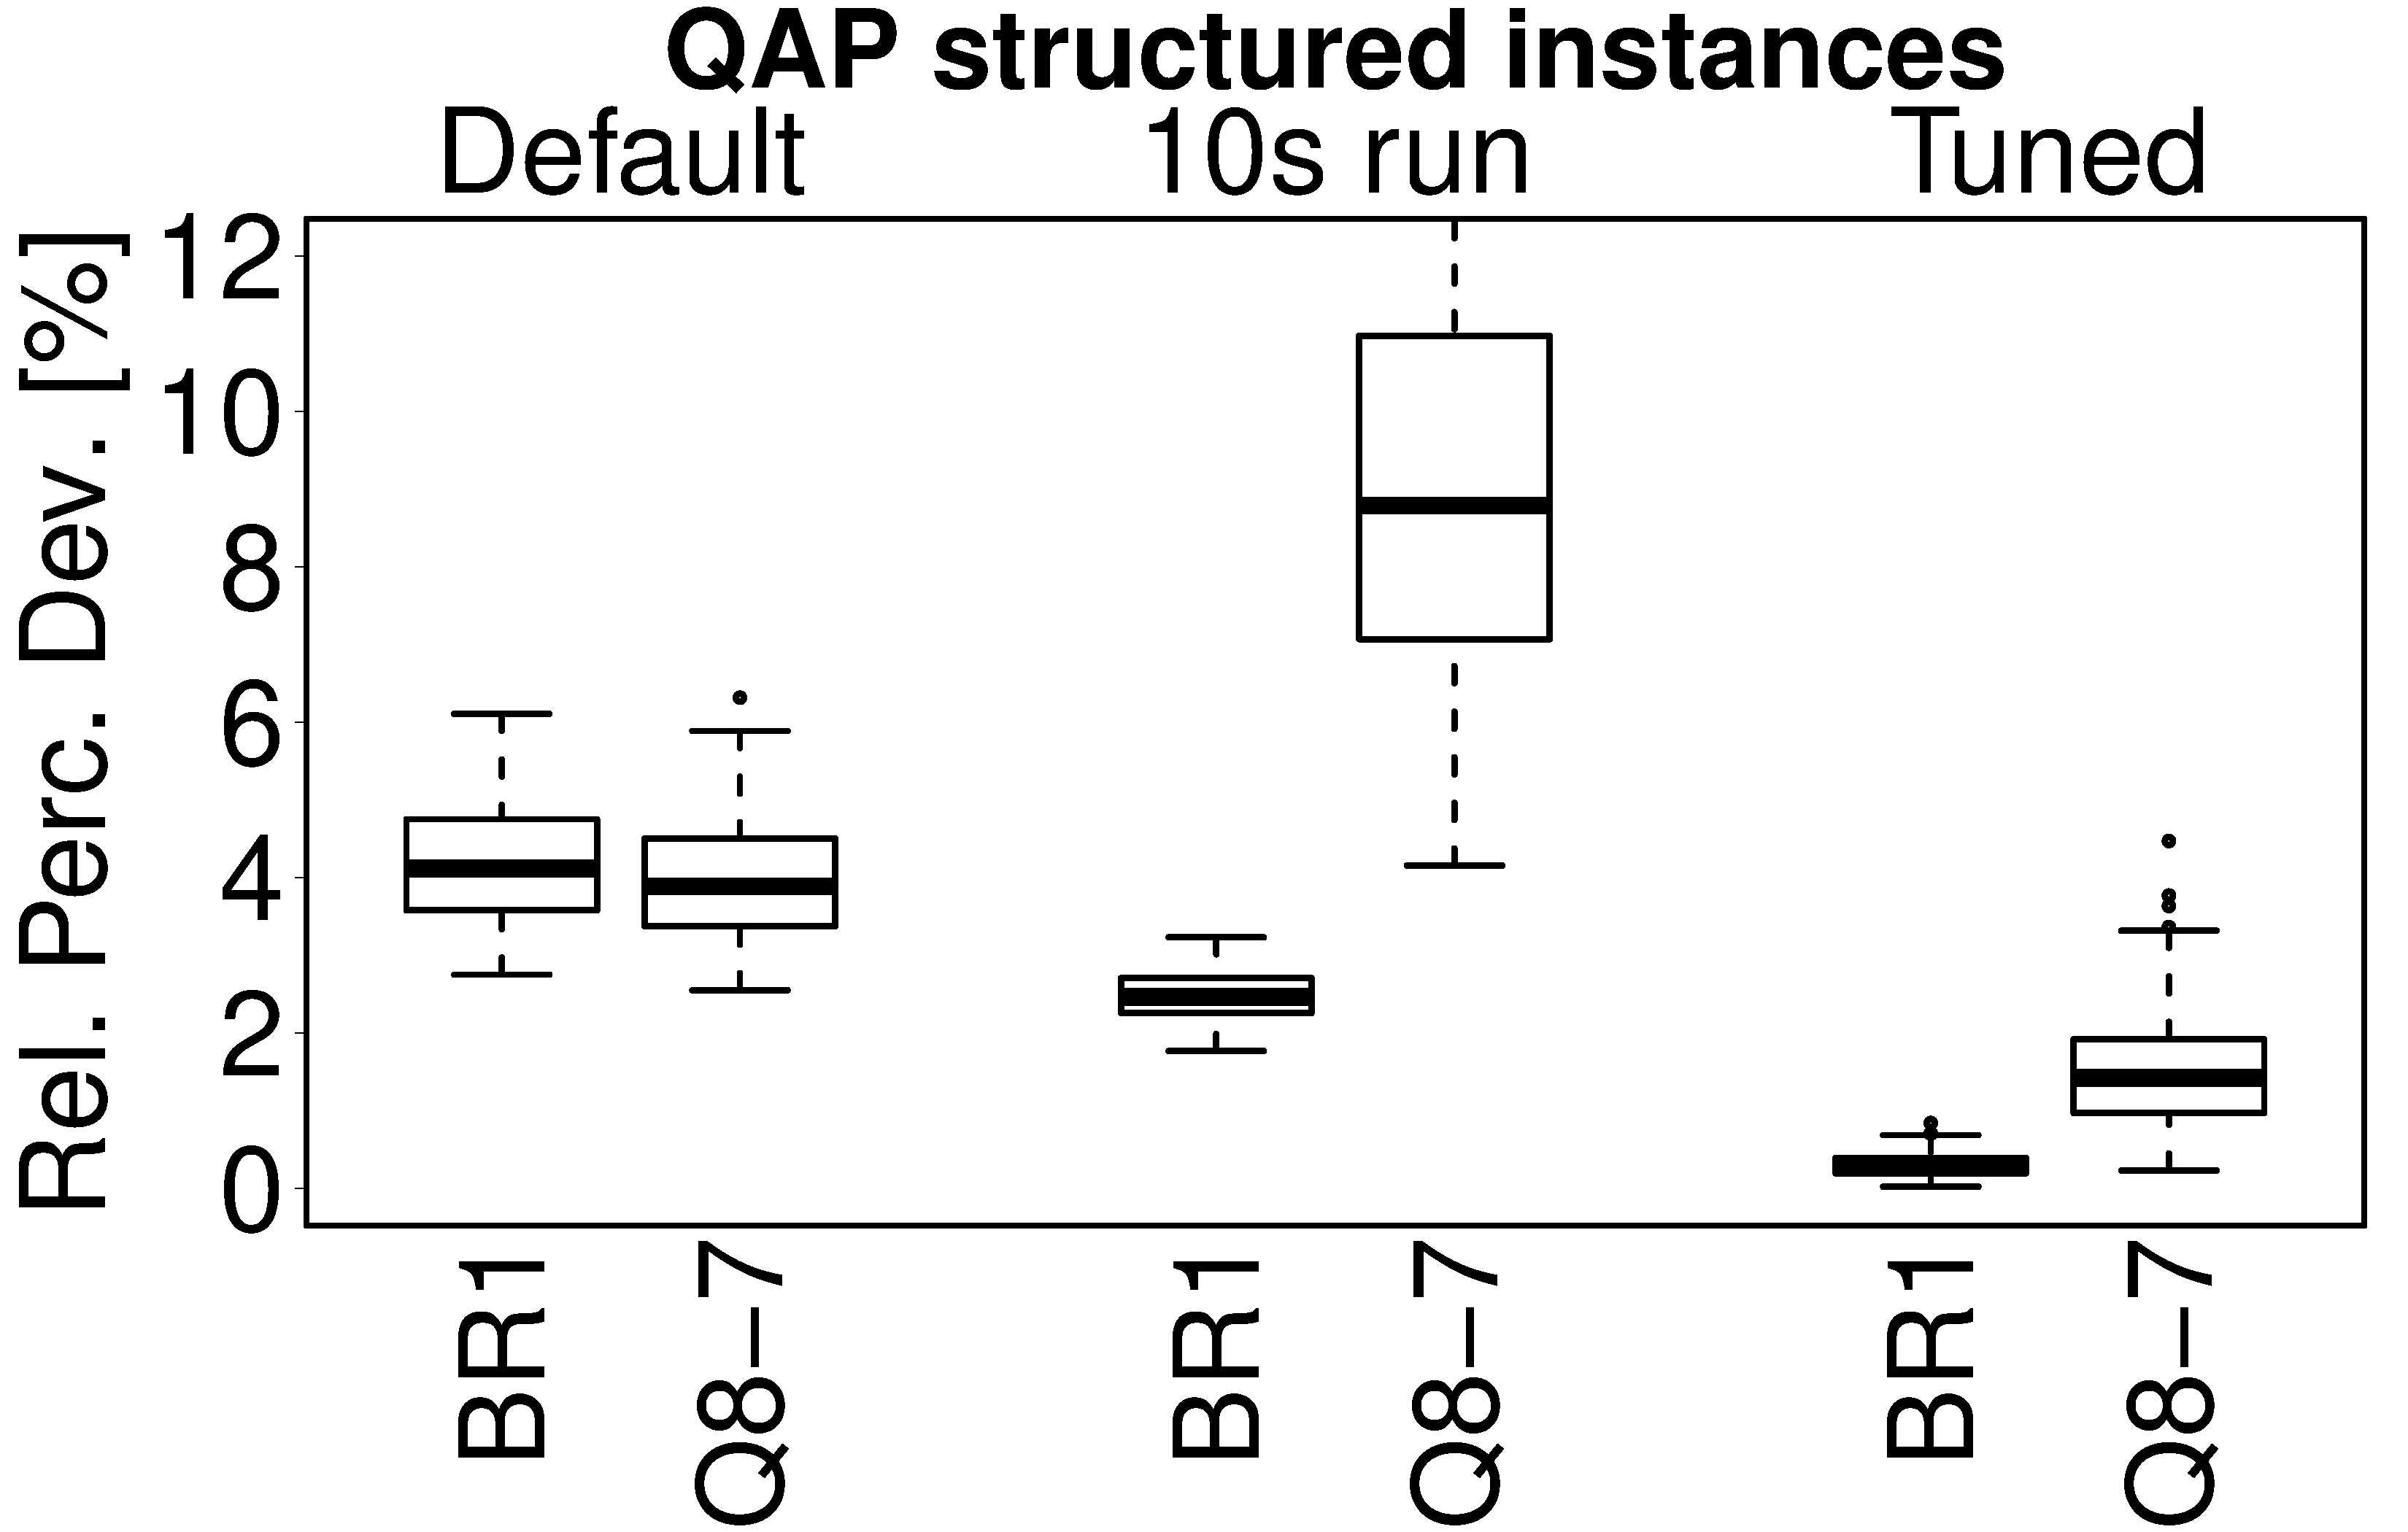
\includegraphics[width=0.49\textwidth]{Part 2 - Search-Based Optimization/Simulated Annealing/figures/es-bxp.pdf}
    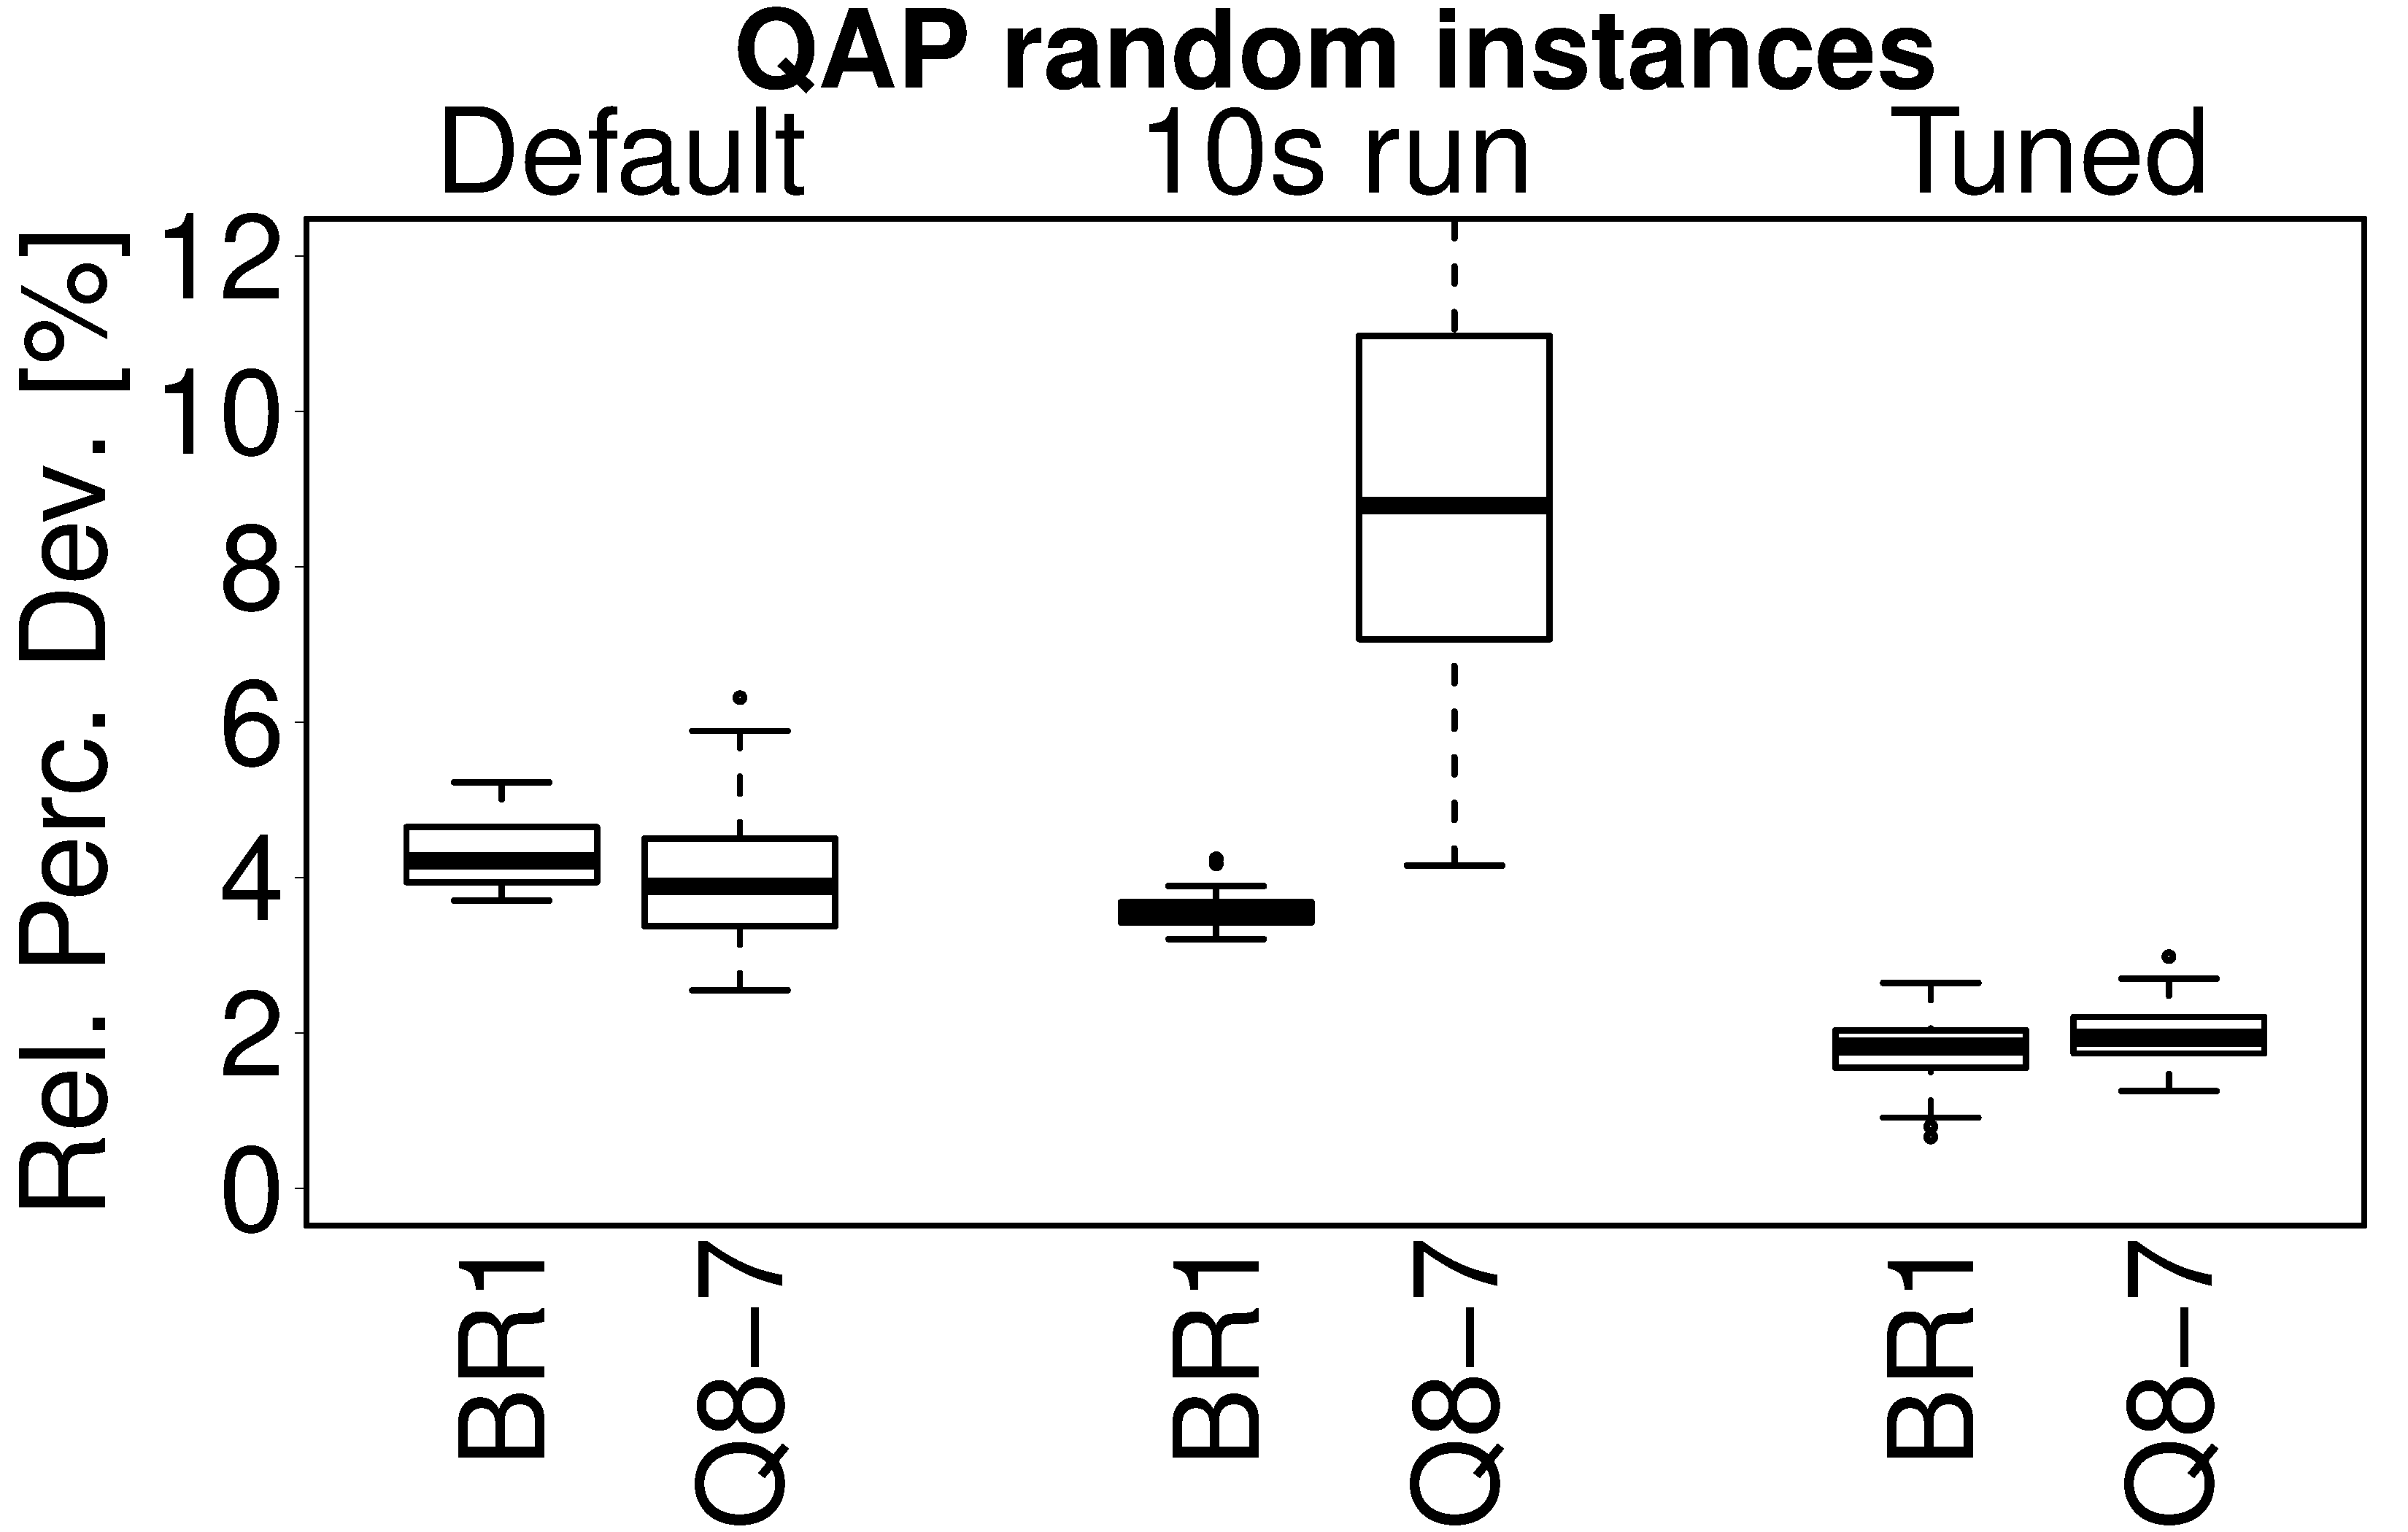
\includegraphics[width=0.49\textwidth]{Part 2 - Search-Based Optimization/Simulated Annealing/figures/rr-bxp.pdf}
  \end{center}
  \caption{Percentage deviation from the best known solutions obtained
  by the two simulated annealing algorithms on our structured
  and random QAP test set in their default settings, when let run for ten seconds,
  and when tuned using irace on a separate training set.}
  \label{fig:resqap1}
\end{figure}

In the first experiment the results obtained by \brsa and \qsa are similar, with a relative percent 
deviation (RPD) around $4\%$. This is because the algorithms are fairly old and 
most likely they have been manually
fine-tuned on small instances with little computational power available. 
If we let them run for a longer time, 
which can be done by simply replacing the termination condition,
this clearly favours \brsa that improves its results. 
The same modification has however a surprising effect on \qsa, which 
significantly worsens its results. This can be explained by considering 
how the Q8-7 cooling scheme is defined in the original paper. When 
this component is re-implemented exactly as described, one of the parameters
is computed relatively to the expected number of total move 
evaluations of the search. This value defines
therefore a delicate balance, that collapses if this value 
increases dramatically, as it is the case in our experiments. The resulting 
value makes therefore the temperature update too slow, and the algorithm
is unable to remain on good converging paths as it has a very high probability
of accepting worsening moves for a too large part of the search. 
We then tune the numerical parameters of the algorithms using irace, paying
attention to modifying the Q8-7 cooling scheme such that its parameters
can be independently configured. In this case, on both instance classes
both algorithms significantly improve their performance. 
On the structured instances, however, \brsa with an RPD of around $0.2\%$ 
clearly outperforms \qsa, which finds solutions on average worse than $1\%$ 
over the best known ones. On the random instances, instead, both algorithms obtain 
solutions on average just below $1\%$ of RPD, with \brsa marginally better than \qsa.

\begin{figure}[tb]
  \begin{center}
    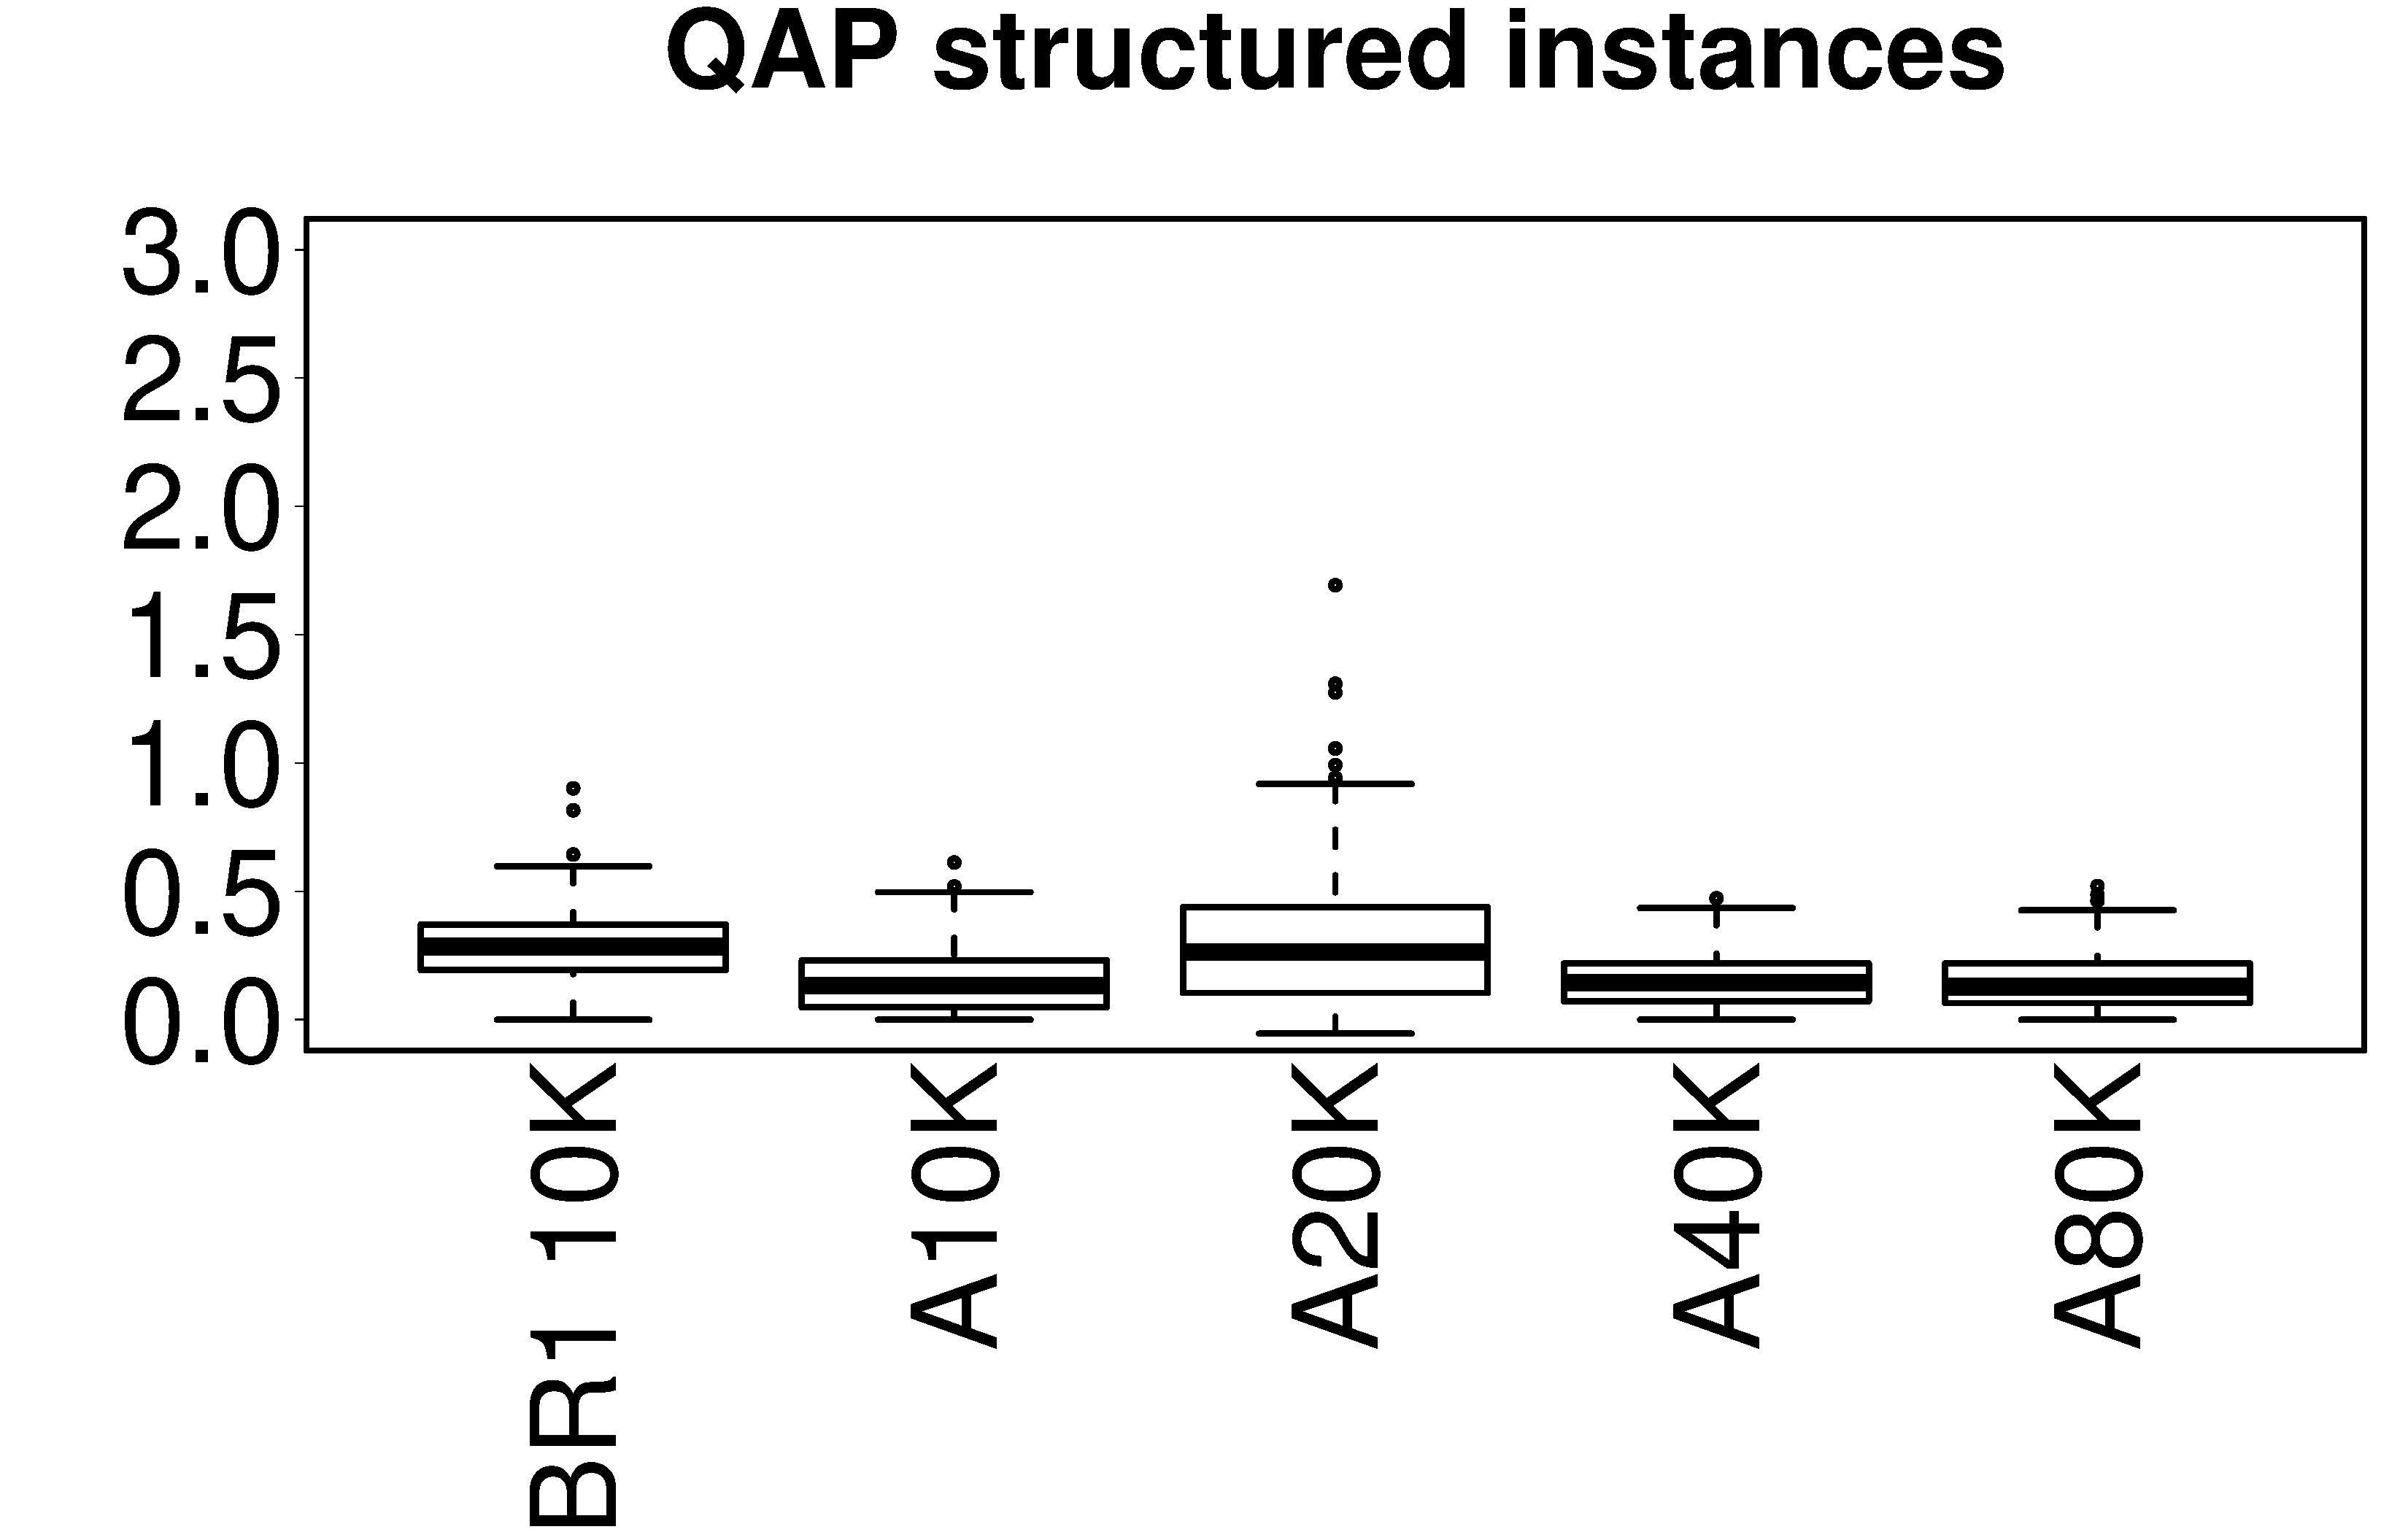
\includegraphics[width=0.49\textwidth]{Part 2 - Search-Based Optimization/Simulated Annealing/figures/esall-bxp.pdf}
    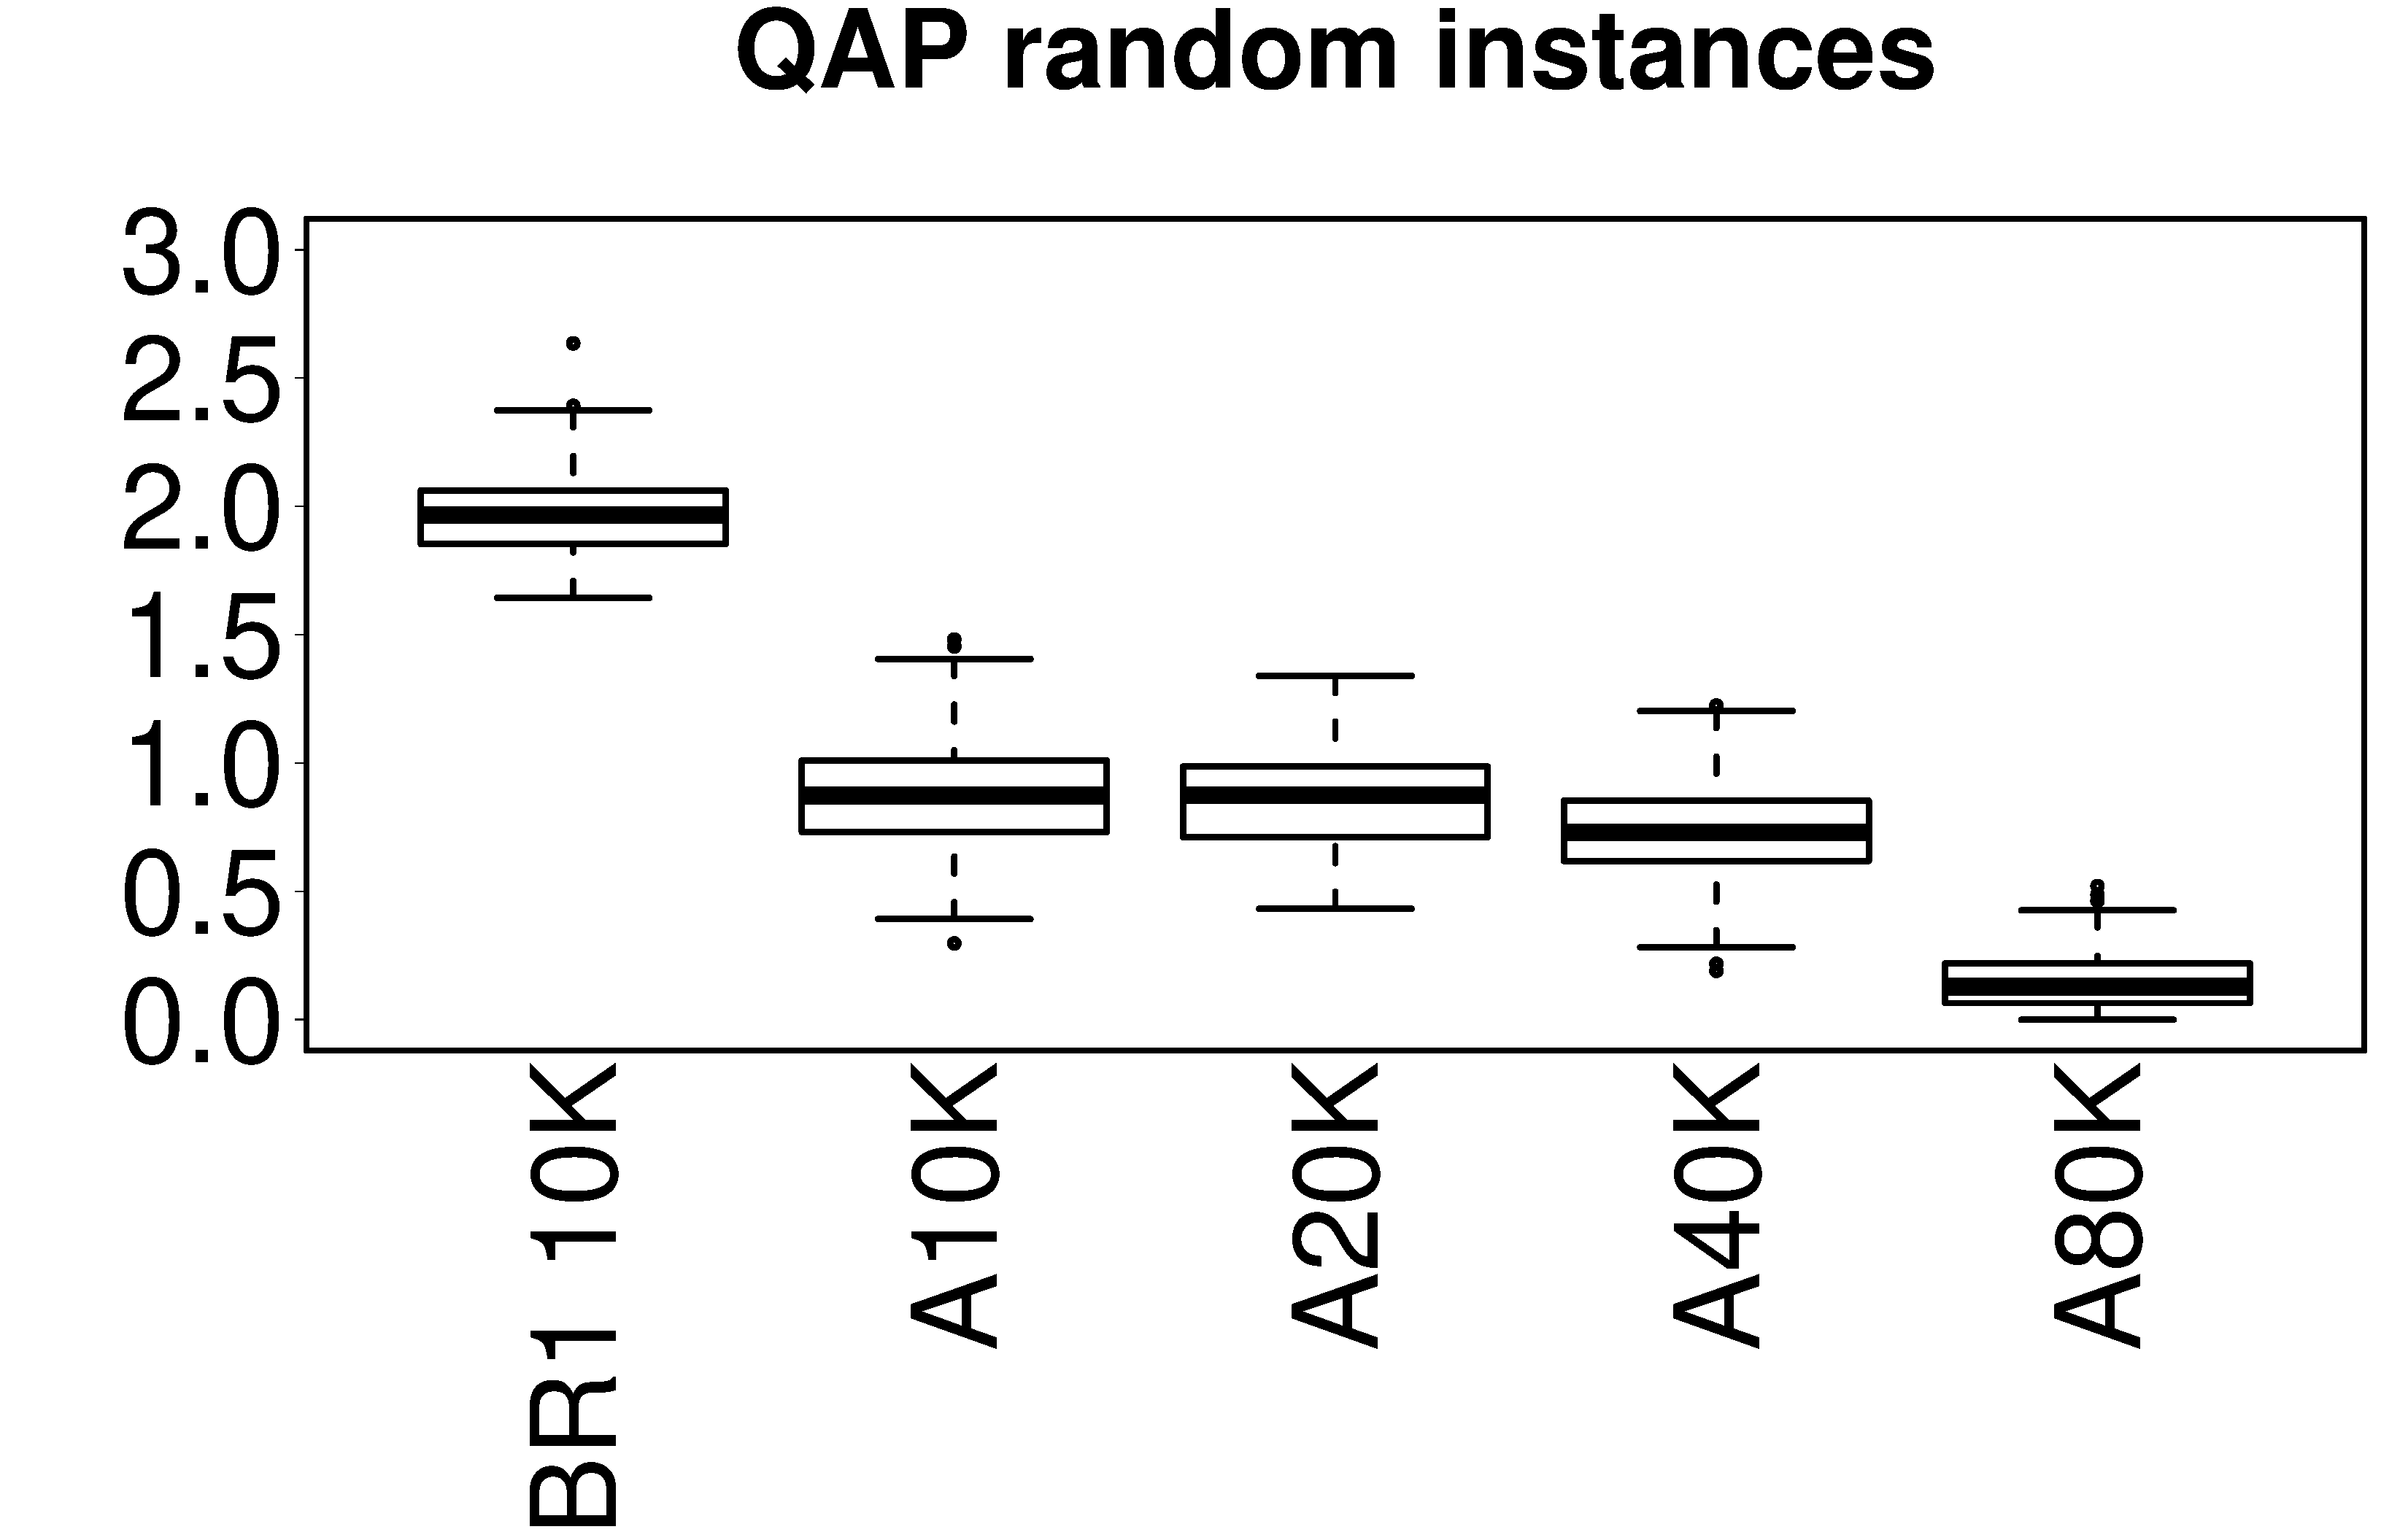
\includegraphics[width=0.49\textwidth]{Part 2 - Search-Based Optimization/Simulated Annealing/figures/rrall-bxp.pdf}
  \end{center}
  \caption{Percentage deviation from the best known solutions obtained
  when automatically designing simulated annealing algorithms from scratch using $10$K, $20$K, 
  $40$K and $80$K experiments on our structured and random QAP test set, compared
  with \brsa tuned with $10$K experiments.}
  \label{fig:res2qap}
\end{figure}


\subsubsection{Generating new algorithms}
Finally, we exploit the whole set of options identified in the literature
for the different simulated annealing components, using irace to automatically select
the best combination and thus design new algorithms from scratch. We report
in Figure \ref{fig:res2qap}
the results obtained by the algorithms that result from automated design tasks
with $10$K, $20$K, $40$K and $80$K experiments.
The algorithms obtained with the highest budget are reported 
in Algorithms \ref{algo:allsaes} and \ref{algo:allsarr} for 
structured and random instances, respectively.


\begin{algorithm}[ht!]
	  \caption{Component-based formulation of the SA automatically designed 
	  for the structured instances with a tuning budget of $80$ thousands experiments. 
	  The components are highlighted in \textit{italic}.}
     \label{algo:allsaes}
    
    Parameters: a problem instance $\mathcal{I}$, the \textit{$2$-exchange neighbourhood}, 
    \textit{a random permutation $\mathbf{x}_0$}, control parameters 
    $\theta = (p, 0.2249, k = 0.6969, \beta = 4645.392, \alpha = 0.6921, \gamma = 32)$
    
    Output: the best solution $\mathbf{x^*}$ found during the search.
    
	\begin{algorithmic}[1] 
		\STATE{$\textrm{best solution } \mathbf{x^*} := \textrm{incumbent solution } \mathbf{\hat{x}} := \mathbf{x}_0$\;}
		\STATE{$i := 0$\;}
        \STATE{Initialize temperature $T_0$ as \textit{the value that gives an expected initial acceptance probability $p$ of worsening moves in a random walk of length $l=10^4$, with a scaling factor $k$} \;}
		\WHILE{\textit{less than $10$ seconds of runtime}}
		\STATE{choose a solution $\mathbf{x}_{i+1}$ in the \textit{$2$-exchange neighbourhood} of $\mathbf{\hat{x}}$ \textit{at random}\;}
		\IF{$ \mathbf{x}_{i+1}$ meets \textit{Metropolis criterion}}
		\STATE{$ \mathbf{\hat{x}} := \mathbf{x}_{i+1}$\;}
		\IF{$ \mathbf{\hat{x}}$ improves over $\mathbf{x^*}$}
		\STATE{$\mathbf{x^*} :=  \mathbf{\hat{x}}$\;}
		\ENDIF
		\ENDIF
		\IF{\textit{the temperature value drops below} $\beta$}
		\STATE{update temperature according to \textit{geometric cooling with factor} $\alpha$\;}
		\STATE{reset temperature \textit{to initial value $\gamma$ times the neighbourhood size}\;}
		\ENDIF
		\STATE{$i := i + 1$\;}
		\ENDWHILE
        \STATE{return $\mathbf{x^*}$\;}
	\end{algorithmic}
\end{algorithm}


\begin{algorithm}[ht!]

	  \caption{Component-based formulation of the SA automatically designed for 
	  the random instances with a tuning budget of $80$ thousands experiments. 
	  The components are highlighted in \textit{italic}.}
     \label{algo:allsarr}
    
    Parameters: a problem instance $\mathcal{I}$, the \textit{$2$-exchange neighbourhood}, 
    \textit{a random permutation $\mathbf{x}_0$}, control parameters 
    $\theta = (k = 0.5438, \delta = 632, \alpha = 0.0.5927, \beta = 0.65, \gamma = 1208, r = 71822, s = 0.0828)$
    
    Output: the best solution $\mathbf{x^*}$ found during the search.
    
	\begin{algorithmic}[1] 
		\STATE{$\textrm{best solution } \mathbf{x^*} := \textrm{incumbent solution } \mathbf{\hat{x}} := \mathbf{x}_0$\;}
		\STATE{$i := 0$\;}
        \STATE{Initialize temperature $T_0$ as \textit{the average gap between consecutive solutions in a random walk of length $l=10^4$, with a scaling factor $k$} \;}
		\WHILE{\textit{less than $10$ seconds of runtime}}
		\STATE{choose a solution $\mathbf{x}_{i+1}$ in the \textit{$2$-exchange neighbourhood} of $\mathbf{\hat{x}}$ \textit{as the best one among $\delta$ randomly chosen ones}\;}
		\IF{$ \mathbf{x}_{i+1}$ meets \textit{Metropolis criterion}}
		\STATE{$ \mathbf{\hat{x}} := \mathbf{x}_{i+1}$\;}
		\IF{$ \mathbf{\hat{x}}$ improves over $\mathbf{x^*}$}
		\STATE{$\mathbf{x^*} :=  \mathbf{\hat{x}}$\;}
		\ENDIF
		\ENDIF
		\IF{\textit{exponentially increasing temperature length with parameters $r,s$} is met}
		\STATE{update temperature according to \textit{geometric cooling variant with factors} $\alpha, \beta$\;}
		\STATE{reset temperature \textit{to the one of the best solution found if no move accepted in the last $\gamma$ ones}\;}
		\ENDIF
		\STATE{$i := i + 1$\;}
		\ENDWHILE
        \STATE{return $\mathbf{x^*}$\;}
	\end{algorithmic}
\end{algorithm}

On the structured instances the results are slightly better than those obtained
by \brsa, with the exception of the configuration found with $20$K experiments.
This is a somewhat easy scenario, and it takes relatively little effort
to find good solutions. 
The random instances scenario is instead more challenging, and it takes 
more experiments to find a suitably good configuration. In fact, while
the tuning with $10$ thousand experiments improves a lot over \brsa,
it takes $40$ thousand experiments to marginally improve the results. Using
$80$ thousand experiments, however, it is possible to find configurations that
find solution qualities comparable to the structured instances case.

For different budgets, the results obtained on the structured instances
are very similar, and so are the algorithms. They all feature original simulated annealing components
such as the Metropolis acceptance, a geometric cooling scheme with cooling rates 
between $0.61$ and $0.83$ and a
random neighbourhood exploration.
There are instead different strategies for the temperature length and restart.
The initial temperature is defined in different ways, all of them relatively to 
some statistics computed during a preliminary random walk in the solution space. 
The algorithms obtained for the random instances are more different among each other.
The only common component is the Metropolis acceptance criterion. 
A closer inspection of the search trajectory reveals instead that
the algorithms effectively maintain the same or almost the same temperature value
for large portions of the search. In other words, the tuning process ends up shaping
a relatively complex algorithm that works like a very simple one. Our set of options
includes the possibility of maintaining the same temperature throughout the whole search, 
but it is more difficult to initially sample one with good settings, that has the chance of
surviving during the tuning.

The difference in the algorithms obtained can be explained with a closer
inspection to the landscapes traversed by the algorithms. On the random instances
the neighbourhoods have a distribution of solution values 
relatively similar to solutions in areas of different quality around the solution space, 
making this a scenario
that does not require variations of the algorithm parameters. On the 
structured instances, instead, neighbourhoods centered around average quality solutions
have different distributions of values than neighbourhoods around good solutions, and in this case
the flexibility of simulated annealing makes it more likely to adapt the algorithm to
the different areas of the landscape encountered \cite{IRIDIA-2021-005}.

It has to be noted that we considered only one tuning task for every budget, and
repeating each task with a different random seed may give algorithms that are different,
to a certain extent. At the same time, we have run the configuration tasks for the algorithm 
that has the full training set of 100 parameters for four different budgets. We commonly observe 
that a higher budget usually is good especially if the configuration tasks have many parameters. 
Anyway, one should observe that on the structured instances with 20K one has a relatively 
poor algorithm, 
something that can happen due to the stochasticity in the configuration process.



\section{Summary and Discussion}
\label{sec:conclusions}

In this chapter, we have seen how to implement a simulated annealing 
algorithm in terms of the design choices to make. 
We have shown how to combine the knowledge on algorithmic components 
and parameter settings  with automatic configuration tools 
to develop efficient simulated annealing
algorithms. This methodology is nonetheless general, 
and works for any stochastic local search method.
There are some inherent advantages 
for this such as making these components and parameters available for 
future use, allowing experimental analyses to identify the circumstances under which
every component will be most successful,
and exploiting directly the recent advances in the automatic 
configuration of algorithms.
This applies even more strongly when we want to design an algorithm that finds
good solutions as soon as possible, or, in other words, that exhibits a good 
\textit{anytime behaviour}. 

In the experiments we observed how good simulated annealing algorithms look 
like for different QAP instance classes.  
In general, in \cite{FraStu2019:cor} we have many more simulated annealing algorithms 
for the QAP identified and, independent of which simulated annealing we have, 
we found the automated configured simulated annealing with the variety of our settings 
always superior to these specifically designed algorithm for the QAP.
An importance analysis conducted across different problems and instance classes
indicated in fact that the acceptance criterion is the most important component in a
simulated annealing, followed by the neighbourhood exploration criterion. 
These two components are precisely the ones that operate locally in the neighbourhood.
In general, we have seen that different scenarios require different algorithms,
but even for the same scenario we may have different algorithms that perform 
equally well. 
Quantifying the appropriate diversification and understanding what algorithm 
could obtain the desired behaviour are anyway tasks 
better performed with the help of automatic tools. They can, in fact, 
select the best options for each algorithmic component and parameter, 
thus making the best out of the available body of knowledge that can be
found in the literature. 

A different approach is extending our approach to other stochastic local search methods and to 
generate extended frameworks. Ideally, these extensions would be 
generated within a same framework so that possibly rich hybrids 
among these methods may be generated. This would enable us to 
compare automatically designed simulated annealings against other automatically 
designed stochastic local searches, to study the role, impact and composition of 
simulated annealing algorithms when combined with or used as part of other 
stochastic local searches. Ultimately, we can try to understand 
when and how to move beyond the simulated 
annealing structure, to automatically design bottom up new methods without 
constraining them to a predetermined form.

\section{Exercise}\label{sec:exercise}
In addition to \brsa and \qsa, in the literature there are several papers
proposing SA algorithms for the QAP or for problems that can be modeled
as such. 
We propose an open-ended exercise to become acquainted not only with 
Simulated Annealing, but also with a component-based perspective
on stochastic local search algorithms, and its automatic optimization.
You can take inspiration from the Supplementary Material of this chapter\footnote{\supplementurlsa}, but you can also start with a new clean implementation.

\begin{enumerate}
    \item Choose a SA for the QAP to implement. You can start from the works we
    cited in this Chapter, or you can look for other SA algorithms.
    \item Identify the components of the algorithm you chose
    comparing it with against the template we provide in Section
    \ref{sec:sacomponents}, along with their numerical parameters.
    \item Understand how they interact: think about each of them as a separate
    function, and analyze which data can be considered \textit{input}
    and \textit{output}.
    Use the template given in Algorithm \ref{algo:simannealing} as a  
    reference to determine the flow of information among the components.
    \item Implement the algorithm, making sure you can specify the 
    numerical values as command line parameters. SA is
    a stochastic algorithm, so remember to
    make it possible to specify a random seed too.
    \item Run some tests on the instances we provide in the Supplementary
    Material\footnote{\supplementurlsa}. Use different random seeds and record the results
    you observe.
    \item Play with the numerical parameters, trying to find
    a parameter combination that performs consistently better than
    the original parameter values.
    \item Use irace and the templates
    provided in the Supplementary Material\footnote{\supplementurlsa} to automatically tune
    the numerical parameters \cite{LopDubPerStuBir2016irace}. 
    Re-run the tests, and observe the difference of results.
    \item If you feel brave, implement alternative components, such as
    new functions to update the temperature value, or to determine 
    whether to accept a candidate solution. You can take these ideas
    from existing papers, or come up with new components on your own.
    An implementation that reflects the component-based perspective
    of SA will make it way easier to observe the impact of your new
    components. You can even introduce a new command line parameter
    to add the choice at runtime.
\end{enumerate}

\section*{Acknowledgments}
Alberto Franzin acknowledges support from the 
Service Public de Wallonie Recherche under grant n\textdegree 2010235 - ARIAC by DIGITALWALLONIA4.AI.
Thomas St\"utzle acknowledges support from the Belgian F.R.S.-FNRS,
of which he is a Research Director. 

\bibliographystyle{unsrt}
\bibliography{bibliography}
